\chapter{Experimentación y Resultados}\label{chapter:implementation}
En este capítulo se exponen los resultados, las ventajas, desventajas y comparaciones de usar la biblioteca \texttt{fabric-chaincode-csharp} con respecto a las implementadas en otros lenguajes.

\section{Ventajas del uso de $ C\sharp $ en Hyperledger Fabric}
La biblioteca propuesta permite la creación de contratos inteligentes en  $ C\sharp $. Como resultado, es posible aprovechar características propias del lenguaje para crear aplicaciones sólidas y duraderas sobre Hyperledger Fabric. Para respaldar esta afirmación se analizarán ejemplos de contratos inteligentes escritos en $ C\sharp $ que implementan la interfaz \texttt{IChaincode} propuesta en la biblioteca \texttt{fabric-chaincode-csharp}.



\begin{figure}[tbph]
\centering
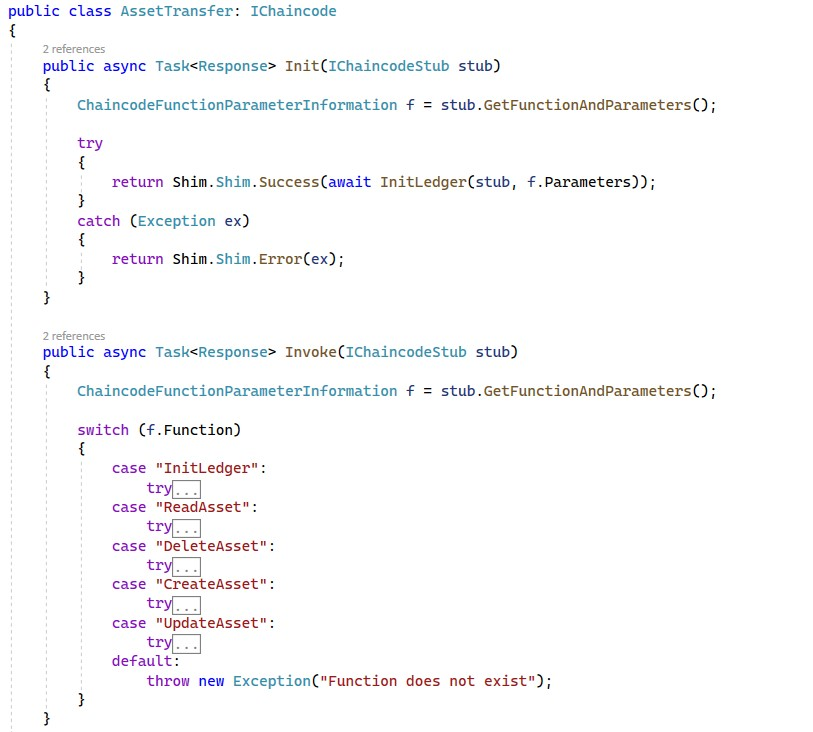
\includegraphics[width=\textwidth]{Images/assettransfer}
\caption{Contrato inteligente \texttt{AssetTransfer}}
\label{fig:assettransfer}
\end{figure}


La figura \ref{fig:assettransfer} muestra el contrato inteligente \texttt{AssetTransfer}, el cual aprovecha las características:

\begin{enumerate}

\item Interfaces. Se emplea la interfaz IChaincodeStub para agrupar las funcionalidades que permiten acceder a los servicios de invocación del ledger. La interfaz IChaincode provee al contrato los métodos que constituyen el punto de entrada para realizar propuestas de transacciones.

\item Soporte del lenguaje para operaciones asíncronas. Permite ejecutar de forma concurrente las funciones que necesitan interactuar con el peer para devolver un resultado, en este caso \texttt{InitLedger}, \texttt{ReadAsset}, \texttt{DeleteAsset}, \texttt{CreateAsset} y \texttt{UpdateAsset}. 

\item Genericidad. Se utiliza \texttt{Task<T>} en los métodos del contrato para representar una operación asíncrona que devuelve un valor de tipo \texttt{T}. Esto facilita la implementación de contratos, pues evita tener que crear una clase que soporte operaciones asíncronas por cada tipo que se quiera retornar.

%Las funciones del contrato que interactúan con el peer deben retornar Task para poder realizarse de forma concurrente.

%Se utiliza en el tipo \texttt{Task<Response>}. Usar un parámetro de tipo genérico, permite escribir una sola clase que otro código de cliente puede usar sin incurrir en el costo o el riesgo de las conversiones en tiempo de ejecución o las operaciones de \textit{boxing}.

\item Manejo de excepciones. Se utiliza la expresión \texttt{try/catch} para lidiar con errores durante la ejecución de una transacción. Permite escribir un código confiable, lo menos propenso a fallos posible.
\end{enumerate}

\section{Experimentación}

Para probar el correcto funcionamiento de la herramienta propuesta, se crearon numerosos contratos inteligentes. A continuación, se analizará un ejemplo.

A partir de la biblioteca propuesta el contrato inteligente \texttt{AssetTransfer} puede interactuar con la red \textit{blockchain} y realizar las operaciones: 

\begin{enumerate}
\item \texttt{CreateAsset}: Añade un elemento al \textit{ledger} a partir de la función del \textit{stub} \texttt{PutState(key, value)}.\\

\begin{lstlisting}[caption={Función \texttt{CreateAsset(...)}}]
public async Task<ByteString> CreateAsset(IChaincodeStub stub, Parameters parameters)
{

    parameters.AssertCount(2);
    string key = parameters[0];
    string value = parameters[1];


    var asset = new Asset(value);
    string jsonString = JsonSerializer.Serialize(asset);

    await stub.PutState(key, ByteString.CopyFromUtf8(jsonString));
    
    return ByteString.Empty;
}
\end{lstlisting}

\item \texttt{ReadAsset}: Devuelve un elemento del \textit{ledger} a partir de la función del \textit{stub} \texttt{GetState(key)}.\\

\begin{lstlisting}[caption={Función \texttt{ReadAsset(...)}}]
 public async Task<ByteString> ReadAsset(IChaincodeStub stub, Parameters parameters)
{
    string key = parameters[0];
    var asset =  await stub.GetState(key);
    if (asset == null || asset.Length <= 0) 
    	throw new Exception ("Asset {key} does not exist.");

    return asset;
}
\end{lstlisting}

\item \texttt{UpdateAsset}: Modifica un elemento del \textit{ledger} a partir de la función del \textit{stub}\texttt{ PutState(key)}.\\

\begin{lstlisting}[caption={Función \texttt{UpdateAsset(...)}}]
public async Task<ByteString> UpdateAsset(IChaincodeStub stub, Parameters parameters)
{
    string key = parameters[0];
    string value = parameters[1];

    var serializedJson = await stub.GetState(key);
    var asset = JsonSerializer.Deserialize<Asset>(serializedJson.ToStringUtf8());
    asset.Value = value;
    
    string jsonString = JsonSerializer.Serialize(asset);
    var updatedAsset = await stub.PutState(key, ByteString.CopyFromUtf8(jsonString));
    
    return ByteString.Empty;
}
\end{lstlisting}

\item \texttt{DeleteAsset}: Elimina un elemento del \textit{ledger} a partir de la función del \textit{stub} \texttt{DeleteState(key)}.\\

\begin{lstlisting}[caption={Función \texttt{DeleteAsset(...)}}]
public async Task<ByteString> DeleteAsset(IChaincodeStub stub, Parameters parameters)
{
    string key = parameters[0];
    await stub.DeleteState(key); 
    return ByteString.Empty;
}
\end{lstlisting}
\end{enumerate}

%Crear, Leer, Actualizar y Borrar, conocidas como operaciones CRUD por sus siglas en inglés.




%En este ejemplo se evidencia el manejo de excepciones y el soporte del lenguaje para operaciones asíncronas. El primero a través de la expresión try/catch y el segundo en el uso de las palabras clave async, await y Task. Sigue lo que se conoce como Patrón Asíncrono Basado en Tareas (TAP)  espera una operación que devuelva una Tarea o Task<T> dentro de un método asíncrono.


%C# tiene un modelo de programación asíncrona a nivel de lenguaje, que permite escribir fácilmente código asíncrono sin tener que hacer malabarismos con las devoluciones de llamada o ajustarse a una biblioteca que admita la asincronía. Sigue lo que se conoce como Patrón Asíncrono Basado en Tareas (TAP). 
%
%El modelo es bastante simple: espera una operación que devuelva una Tarea o Task<T> dentro de un método asíncrono.
%
%El núcleo de la programación asincrónica son los objetos Task y Task<T>, que modelan operaciones asincrónicas.
%
%La palabra clave async convierte un método en asíncrono, lo que le permite usar la palabra clave await en su cuerpo.
%
%Cuando se aplica la palabra clave await, suspende el método de llamada y devuelve el control a la persona que llama hasta que se completa la tarea esperada.




%$ C\sharp $ es un lenguaje orientado a objetos. Este paradigma de la programación fomenta la productividad en el desarrollo de \textit{software} mediante las propiedades: encapsulación, herencia y polimorfismo. La primera consiste en la posibilidad de una clase o estructura de especificar qué tan accesible es cada uno de sus miembros. La herencia es útil cuando se necesita agregar funcionalidad a un tipo existente. El polimorfismo permite que en tiempo de ejecución, los objetos de una clase derivada pueden tratarse como objetos de una clase base en lugares como parámetros de método.

%Otras facilidades que provee el lenguaje $ C\sharp $ incluyen:
%
%\begin{enumerate}
%\item Las expresiones \textit{lambda} admiten técnicas de programación funcional.
%
%\item  Admite tipos por referencia y por valor definidos por el usuario. 
%
%\item  Los tipos anulables protegen contra variables que no hacen referencia a objetos asignados.
%
%\item El manejo de excepciones proporciona un enfoque estructurado y extensible para la detección y recuperación de errores.
%
%\item El soporte de lenguaje para operaciones asíncronas proporciona sintaxis para construir sistemas distribuidos.
%\end{enumerate}

Si se compara con \texttt{fabric-chaincode-go} la biblioteca propuesta tiene como ventaja la capacidad de crear procesos concurrentes dentro de una misma transacción. Esto gracias a la implementación de la clase \texttt{MsgQueueHandler}, la cual maneja la interacción con el \textit{peer} a través de un diccionario que asocia a cada transacción una cola de mensajes. De esta forma, pueden existir varios hilos dentro del contexto de una misma transacción pues, el intercambio con el \textit{peer} se realiza de forma síncrona en el orden en que se añaden los mensajes en la cola.

%Aparte de las ventajas mencionadas, también existen limitaciones.
%La \texttt{fabric-chaincode-api} propuesta no implementa todas las funcionalidades que existen en el resto de bibliotecas. Por ejemplo, en Javascript/Typescript la \texttt{ChaincodeStubInterface} expone varios métodos que posibilita recibir una secuencia de datos del peer. Esta capacidad es útil pues permite, entre otras cosas, obtener un rango de llaves que cumplen con un determinado criterio o la recuperación de los cambios históricos realizados en el valor asociado a una llave.



%\colorbox{lightgray}{PENDIENTE: Insertar código}
%
%\section{Recomendaciones}



%La implementación de esta capacidad se basa en iteradores. Se definen tres tipos diferentes:
%
%CommonIteratorInterface: define las operaciones comunes de todos los tipos de iteradores.
%
%StateQueryIteratorInterface: especializa la interfaz del iterador base para iterar sobre una colección de claves en el ledger.
%
%HistoryQueryIteratorInterface: esta interfaz especializa la interfaz del iterador base para iterar sobre el historial de cambios de una llave.




